\section{ฟังก์ชันของการแปรผันที่มีขอบเขต}
\textcolor{red}{ยังไม่ได้แก้ไข} 

\hspace{1cm} เมื่อใช้วิธีการแปรผันจนได้สมการอนุพันธ์ย่อยแล้ว จะพบว่าสมการอนุพันธ์ย่อยนั้น เป็นปัญหาค่าขอบ (boundary value problem) ซึ่งจะมีเงื่อนไขเพิ่มเติมเป็น ค่าขอบ (boundary value) ตัวอย่างเช่นเมื่อ $\Omega = [0,1]^2$ และ $u=u(x)$ และสูตรการแปรผัน (varational fomular) เป็น 
\begin{align*}
    \underset{u}{{min}} \int_{\Omega} |\nabla u |^2 dx
\end{align*}

เมื่อใช้วิธ๊การแปรผันแล้วจะได้ปัญหาค่าขอบ

\begin{align*}
\left \{ \begin{array}{ll}  - \triangle u = 0,  & \hspace{1cm} x \in \Omega \\ \dfrac{\partial u}{\partial n} = 0, & \hspace{1cm} x \in \partial \Omega \end{array} \right .
\end{align*}

\hspace{1cm} ซึ่งปัญหาค่าขอบที่ดังที่ได้ยกตัวอย่างให้เห็นนี้เป็นปัญหาค่าขอบแบบนิวแมน (neuman) เนื่องจาก $\dfrac{\partial u}{\partial n} = 0$ ซึ่งค่าขอบแบบนิวแมนนี้เอง จะเป็นสิ่งที่ใช้ในโครงงานวิจัยเรื่องนี้ โดยจะสามารถสร้างค่าขอบนิวแมนได้โดยการขยายโดเมนออก จากนั้นให้ค่าของฟังก์ชันในโดเมนที่ถูกขยายมีค่าเท่ากับค่าที่ใกล้ที่สุดเมื่อวัดระยะทางด้วยระยะทางแบบยูคลิด ดังภาพ \ref{figure:boundary_condition} โดยภาพซ้ายจะมีโดเมนอยู่ในช่วง $[1,8]^2$ ซึ่งการคำนวณบางอย่างเช่นการหาแกรเดียนจำเป็นต้องใช้ค่าขอบเพื่อคำนวณ จึงทำการขยายโดเมนเป็น $[0,9]^2$ โดยจะขยายบริเวณสีแดงที่เป็นขอบในภาพออกไป โดยใช้ค่าที่ใกล้ที่สุดที่อยู่ในขอบสีแดง

\begin{figure}[H]
    \centering
    \begin{subfigure}{0.4\linewidth}
        \centering
        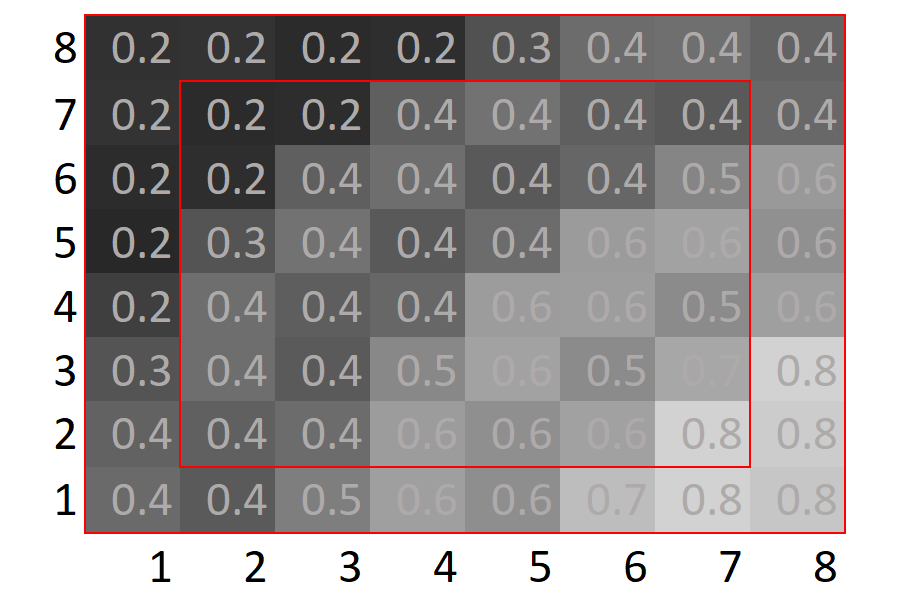
\includegraphics[width=0.8\linewidth]{image/boundary_condition/show_bounary.png}
    \end{subfigure}
    \begin{subfigure}{0.4\linewidth}
        \centering
        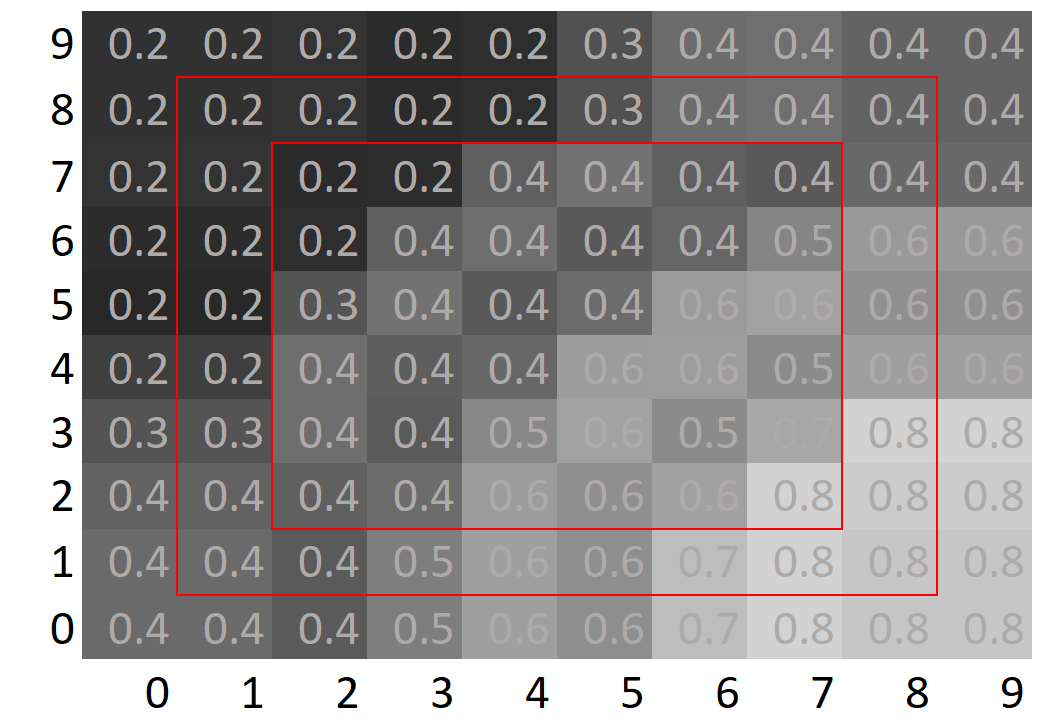
\includegraphics[width=0.8\linewidth]{image/boundary_condition/extend_edge_neuman.png}
    \end{subfigure}
    \label{figure:boundary_condition}
    \caption{ตัวอย่างภาพขอบเขตแบบนิวแมน}
\end{figure}

